
\providecommand{\myrootdir}{..}
\documentclass[\myrootdir/main.tex]{subfiles}

\begin{document}

\chapter{Background and Related Work}
\label{sec:rw}
This chapter presents various research works adjacent or foundational to our work.
The first section presents existing work in the field of continuous integration (CI) and showcases how researchers analyze build logs.
In the second section we describe the existing methods which are the foundation for the chunk retrieval we investigate.
% moritz: nice formulation :)

\section{Continuous Integration and Build Logs}
We describe existing studies about CI to show that CI is a relevant topic within the software engineering research community.
We explain how researchers gather information about CI usage in software projects through build log analysis and why the chunk retrieval techniques we investigate simplifys their data collection.
This section moves on to past works about augmenting build logs to make it easier for developers to inspect them.
The presented approaches are related to and can benefit from the techniques we analyze in this thesis.
Further, we classify build logs as semi-structured data and differentiate our work from system log analysis.
% CI describes the practice of integrating, building and testing source code changes often and fast.
% The tools involved in a CI build communicate their progress and status through a combined build log.
% In Section~\ref{sec:bl-characteristics}, we describe CI builds and how 

% We investigate different techniques which developers and researchers can employ to retrieve information from CI build logs.
% In this section we present 

% research about CI to show that it is a relevant topic in research

% explain methods of those researchers, how they analyzed build logs and how the chunk retrieval techniques we investigate can support them.

% we present existing research into analyzing verbose build logs to help developers intercating with them.

% Following we classify build logs as semi structured data.  and differentiate our work from system log analysis.

\subsection{Continuous Integration}
\label{sec:rw-ci}
The first paragraphs of this section present the results of past research into CI: its influence on the software engineering processes, the reasons for CI builds to fail and the role of testing and of static analysis in CI builds.
Later we describe how researchers obtain the data sets these works are based on.
We show how they analyze build logs and why the chunk retrieval techniques we investigate can support them to broaden their studies.
% This section starts with an overview on research into why CI is used and its impact on development.
% It presents analyses on why CI builds fail and how testing and static analysis tools are used within CI\@.
% We explain how researchers compose data sets for their work on CI and how chunk retrieval techniques can support them.

\paragraph{Motivation for CI and Impact of CI}
Why teams choose to use CI and its impact on the software development process is explored by several existing works.
Hilton et al.~\cite{hilton2017trade-offs} investigate the motivations of developers to use CI through several surveys.
They find that, developers use CI to ensure consistency and quality across different execution environments and increase confidence in the code they deploy.
Hilton et al.~\cite{hilton2016usage} also analyze how and why open source projects use CI\@.
They observe CI usage in a broad range of projects, it supports developers to catch bugs earlier and to shorten release cycles.
Stahl and Bosch~\cite{staahl2014modeling} provide a review of literature on automatic build environments in industry projects.
They propose a descriptive structure to model build flows, which they found to be highly different from project to project.
Vasilescu et al.~\cite{vasilescu2015quality} analyze a broad rage of open source projects written in popular languages on GitHub.
They compare the usage of CI with the successful merges of pull requests and find that CI increase the number of successful merges and allows the team members to uncover more bugs.
In a recent study, Vasallo et al.~\cite{vassallo2019every} interview developers on how they determine why a CI build failed and model how these developers resolve failures.
Vasallo et al. find that, the first and most important steps when developers want to fix a build failure is to locate the error within the build log.
Then the developers use the additional information provided with and around the error message to understand the details of the failures.
This shows that the build log is a central source of information about a CI build.
% Vassallo et al.~\cite{vassallo2018continuous} conducted a survey study on how ci influences developers to continuously refactor their code to fix ci quality analysis warnings.
% Their results indicate that refactoring is rather spread in the ci environment and deemed important by the surveyed developers.
% ``Lack of time'' and ``absence of a proper test suite'' are named as the main barriers to continuous refactoring.
% Vassallo et al.~\cite{vassallo2019automated} analyzed build logs, source code repository content and build metadata of open source repositories for CI anti-patterns.

\paragraph{Build Failures in CI}
Various researchers look into why CI builds fail and into the impact of build failures on the development workflow.
Seo et al.~\cite{seo2014programmers} find that a small group of error types such as dependency mismatches are the most prominent cause of build failures at Google.
In addition, they notice that most failures are resolved within two builds.
Rausch et al.~\cite{rausch2017empirical} analyze CI builds of open source Java projects and find that most builds fail because of failing tests.
For most projects, over half of the failed builds follow a previous failed build.
Rausch et al.'s data shows that most failures occur in the second half of the build runtime, which can cause long delays in the feedback loop, especially when builds are automatically retried upon failure.
Vassallo et al.~\cite{vassallo2017a-tale} compare open source projects in Java to industrial ones.
They determine that testing failures are more common than compilation errors.
Open source builds fail most often because of unit tests, whereas release preparations are the primary cause in industrial projects.

\paragraph{Static Analysis and Testing in CI}
Automated static analysis tools are the focus of Zampetti et al.~\cite{zampetti2017open} in their study of Java projects from GitHub.
Their results show that static analysis is responsible for a small amount of build failures and mainly responsible for warned builds.
Almost all analyzed projects use custom configurations for the static analysis, however the configuration rarely changes.
Failures because of static analysis warnings are observed to be fixed in a short time frame.
Beller et al.~\cite{beller2017oops} show that testing is central to continuous integration when evaluating Travis CI logs for Java and Ruby builds.
They observe a high variation between programming langues, in the kind and number of tests which are run, as well as how often tests fail.
The low failure rates on the CI server hint at code being tested before it is sent to the server.

\paragraph{Data Sets Powering CI Research}
The works presented in this section are based on either developer surveys or data setsa containing build metadata or build logs.
Seo et al.~\cite{seo2014programmers} and Vassallo et al.~\cite{vassallo2017a-tale} based their analyses on sets of build logs collected from industry partners.
Beller et al.~\cite{beller2017travistorrent} created the \emph{TravisTorrent} data set providing access to build metadata from more than 1,000 projects from Travis CI~\cite{travisci2019webpage}.
\emph{TravisTorrent} was the basis for several of the works mentioned in this section~\cite{rausch2017empirical,zampetti2017open,vassallo2017a-tale,beller2017oops}.
Ghaleb et al.~\cite{ghaleb2019studying} aim to identify noise in build breakage data.
They classify build failures from \emph{TravisTorrent} according to whether they were caused by an environmental failure or caused by a developer change.
They also identify cascading build failures created by existing unfixed errors and allowed failures, whose results were later labeled by developers to be ignored.
About half of the failed builds in \emph{TravisTorrent} fall into at least one of these categories.
When regarded as noise they considerably impact observations reported by other works modeling build breakages.

\paragraph{Build Log Analysis in CI Research}
Several of the works we mentioned until now analyze build logs to obtain information about the CI builds. 
For Seo et al.~\cite{seo2014programmers} the build logs are the primary data source for their study.
They develop a custom parser to classify error messages reported by Java and C++ builds. 
Vassallo et al.~\cite{vassallo2017a-tale} analyze collected build logs by extracting error messages using regular expressions.
The regular expressions search for keywords identified in a manual analysis.
The analysis of Ghaleb et al.~\cite{ghaleb2019studying} starts with manual categorization of build logs.
They select keywords and strings that identify their targeted categories and code a script to automatically classify logs based on these keywords.
%To validate the script results, they performed another manual classification.
Beller et al.~\cite{beller2017oops} focus their analysis on Java and Ruby build logs for which they build custom parsers with regular expressions to extract the reason a build failed.

\paragraph{Supporting Log Analysis with Chunk Retrieval}
To leverage the valuable information within build logs the researchers presented in this section build parsers and regular expression-based programs.
This task of retrieving specific chunks of text from the build logs can be solved by the chunk retrieval techniques we compare in this thesis.
Our results can support researchers in choosing a suitable technique for their data set of build logs and the chunks they want to retrieve.
By relieving them from building custom parsers we enable them to cover a much wider range of languages and build tools in their studies.

\subsection{Augmentation of Build Logs}
\label{sec:rw-bl-analysis}
Build logs are a valuable data source for developers to find out why their build failed.
Several researchers are looking into supporting developers to process the verbose build logs.
Vassallo et al.~\cite{vassallo2018un-break} try to shorten the time it takes developers to understand build logs.
They parse Maven~\cite{maven2019website} build logs into a structured representation and create hint generators.
The hint generators leverage this structured access to the information within the build log to propose fixes.
For example, one of the hint generators queries stack overflow for discussions related to why the build failed.
In a qualitative study they observed that highlighting the locality and context of an issue is helpful to programmers.
Their tool BART is published as a Jenkins Plugin~\cite{bart2019plugin}.
The chunk retrieval techniques we compare in this thesis can be used to fill similar structured representations with information from build logs.
As they simplify the construction of parsers they would enable developers and researchers to cover a wider array of build tools, which is the main influence factor on the structure of a build log.

Amar et al.~\cite{amar2019mining} compare different approaches to reduce the portions of a log that a developer has to inspect.
Their techniques remove lines that appear both in logs from passing and failing builds and use a modified \emph{Term Frequency Inverse Document Frequency} (TF-IDF) weighting to identify term vectors likely to occur with failures.
Their diff technique can be interpreted as a chunk retrieval technique, where the targeted information is defined by the past failures used as basis for the weighted term vectors.

Travis itself already provides build log augmentation in the form of a basic structuring of the build logs within their log viewer using \emph{log folds}~\cite{travis2019logfolds}.
They add fold identifiers around common commands and setup or teardown build phases and collapse the contained lines by default.

\subsection{Build Logs as Semi-Structured Data}
\label{sec:rw-semi-structured-data}
Serge Abiteboul introduces a theory of semi-structured data in his report from 1997 about integrating data from several sources~\cite{abiteboul1997querying}.
He proposes essential characteristics of semi-structured data.
In this section, we show how five of these map to the context of build logs.

The structure of build logs
\begin{itemize}
  \item \textbf{is implicit}.
  We might not have access to explicit structuring elements or an explicit structure description.
  Computation is required to infer the present structure.
  \item \textbf{is irregular}.
  Changes in the build process or execution environment might change the structure of a build log.
  We observed this in the logs we collected for the \emph{LogChunks} data set, where for the same repository and build configuration some logs had double new line characters without any noticeable explanation.
  Figure~\ref{fig:log-4} and Figure~\ref{fig:log-5} present an example of this.
  \item \textbf{is partial}. Some parts are highly structured by e.g.\ special characters. Other parts are unstructured, such as natural language text in error messages.
  \item can be described with an \textbf{analytical data guide} rather than a predefined schema.
  There is no fixed specification on how build tools structure their output.
  We later extract structuring patterns in the produced output.
  \item \textbf{has a rapidly evolving schema}.
  Modifications in the build configuration can change the tools involved in the build and therefore the composition of the build log.
  Previous work indicates that some projects change their CI configuration often~\cite{hilton2016usage} and software tools adapt their log messages over time~\cite{yuan2012characterizing}.
\end{itemize}

Abiteboul proposes an approach to overlay the semi-structured data with a structured layer.
The additional layer can answer queries and give access to the semi-structured data relevant to a query.
In contrast to that, this thesis takes a look at techniques to gather a specific, pre-specified information without the need to parse, understand or estimate the whole structure of a log.

\begin{figure}[H]
	\centering
	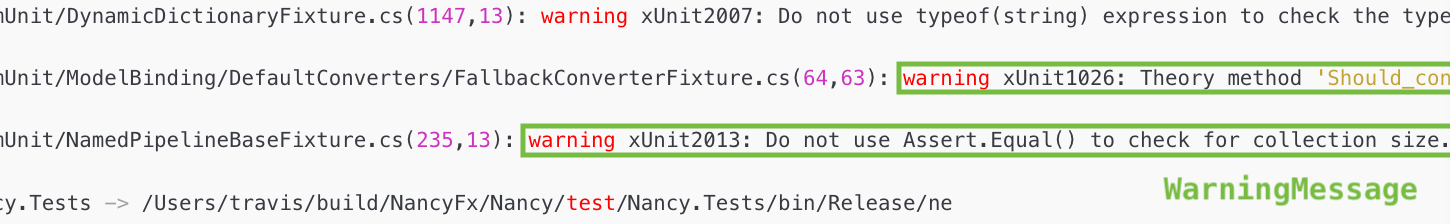
\includegraphics[width=\textwidth, clip]{img/log42.png}
	\caption{Excerpt from a build log showing a WarningMessage chunk.}
	\label{fig:log-4}
\end{figure}
\begin{figure}[H]
	\centering
	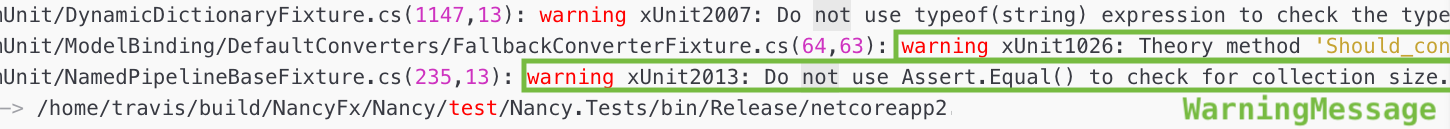
\includegraphics[width=\textwidth, clip]{img/log52.png}
	\caption{Excerpt from a build log showing a differently formatted WarningMessage chunk.}
	\label{fig:log-5}
\end{figure}

\subsection{System Log Analysis}
\label{sec:log-analysis}
A related field of log processing is the processing of system log files produced during runtime.
A main difference between build logs and system logs is that system logs are fundamentally structured through events.
Each line in a log file represents one event with a set of fields: timestamp, verbosity level and raw message content~\cite{he2017towards}.
Figure \ref{lst:system-log} shows example lines from a system log.

The first goal in parsing system log files is to separate constant and variable parts within a log message~\cite{nagappan2010abstracting,he2017towards}.
Next, the log messages are clustered into log events, unifying messages with identical constant parts and varying parameters.
The output of a log parser is a structured log, composed of a list of timed events and the corresponding parameter values~\cite{he2016evaluation}.
This structured log is then the input to various machine learning and data mining processes.
Researchers mine patterns for operational profiling~\cite{nagappan2009efficiently}, debugging~\cite{oliner2012advances}, performance analytics or anomaly detection~\cite{nagappan2010abstracting}.
Xu et al.~\cite{xu2009detecting} leverage the connection of log statements to the source code producing them to separate messages into constant and variable parts more accurately.

The techniques developed for system log analysis can also be applied to build logs.
One example is comparing execution traces to reference traces of intended behavior to detect anomalies.
Amar et al.~\cite{amar2019mining} employed a similar approach to detect relevant lines in build logs.

Classic log parsers interpret the whole log file into a sequence of events.
A similar approach could also be applied to build logs to determine the sequence of executed build steps or phases.
In this thesis we take a different approach and focus on extracting a single specified information from the build log as a whole with chunk retrieval techniques.
Chunk retrieval techniques are used as a part of log parsing to retrieve the values of variable parts in a log message, e.g.\ by using regular expressions~\cite{nagappan2010abstracting,xu2009detecting}.

\lstset{
  morekeywords={INFO, WARN, 2008-11-09},
  postbreak=\mbox{\textcolor{cyan}{$\hookrightarrow$}\space},
  showspaces=false,
  showstringspaces=false,
  keywordstyle=\color{blue},
	frame=single,
  extendedchars=false,
  texcl=false
}
\begin{figure}[]
  \centering
  \begin{lstlisting}[breaklines=true]
2008-11-09 20:46:55,556 INFO dfs.DataNode$Packet- Responder: Received block blk_3587508140051953248 of size 67108864 from /10.251.42.84
2008-11-09 20:49:46,764 WARN PacketResponder 0 for block blk\_3587508140051953248 terminating
  \end{lstlisting}  
  \caption{System Log Statements. Example adapted from~\cite{he2017towards}.}
  \label{lst:system-log}
\end{figure}

\section{Foundational Techniques}
% \section{Information Extraction and Retrieval Techniques}
The techniques we investigate are based on existing methods of Programming by Example, information extraction and information retrieval.
This section presents different Programming by Example resources surrounding the PROSE library.
We explain its generic program synthesis algorithm and how PROSE synthesizes text extraction programs, the foundation of PBE\@.
In addition, we describe how chunk retrieval can be employed as a part of presented information extraction approaches.
We introduce how information retrieval techniques, the basis for CTS, are used to improve software development.

% The chunk retrieval techniques we compare in this thesis use different techniques from the fields of information extraction and retrieval.
% This section presents existing approaches to extract structured information from semi-structured data and how these approaches differ from chunk retrieval.
% Further we illustrate how information retrieval techniques, basis for our chunk retrieval technique CTS, are used in software engineering research.

\subsection{Program Synthesis by Example}
\label{sec:rw-prose}
Programming by Example enables end users to automate repetitive tasks.
The user provides examples for the input and the corresponding output and a synthesis algorithm tries to create the program intended by the user.
This section introduces the theoretical foundations of the program synthesis algorithm of the \emph{Program Synthesis using Examples} (PROSE) framework~\cite{prose2019webpage}.
The PROSE framework is developed by Microsoft Research.
Next, this section presents the FlashExtract DSL, which defines text extraction tasks within PROSE and is the basis for the implementation of our chunk retrieval technique PBE\@.
Finally, we cover additional applications and extensions of the PROSE program synthesis and alternative research on generating regular expressions from examples.

\paragraph{FlashMeta: Inductive Program Synthesis}
The FlashMeta framework presented by Polozov and Gulwani~\cite{polozov2015flashmeta:} is the backbone of the program synthesis in the Microsoft PROSE framework.
FlashMeta separates the inductive synthesis algorithm from the domain specific capabilities of the desired program by encoding the possible program space in a domain specific language (DSL).
The user specifies the desired program behavior by providing in/output examples (I/O examples).
FlashMeta uses \emph{witness functions}, provided by the DSL, to divide the synthesis into smaller subtasks.
For each of these subtasks it enumerates all possible programs that solve the subtask consistent with the set of I/O examples.
A program is consistent with a set of I/O examples if, for each input example, it produces the corresponding output~\cite{mitchell1982generalization}.
The possible subprograms are joined and stored in a \emph{version space algebra} (VSA)~\cite{mitchell1982generalization}.
This a tree structure, which space-efficiently saves candidate programs for tasks by sharing common subexpressions.
Next, FlashMeta ranks the enumerated programs according to which ones the user most likely intended.
The DSL also provides the ranking characteristics.
From the ranked VSA, FlashMeta can then return a ranked list of complete programs consistent with the user's example.

In addition to I/O examples of the intended program, the user can also provide examples with only input or negative input examples.
Negative input examples should not be processed by the synthesized program.

The different applications of PROSE presented in the following paragraphs were all eventually implemented as DSLs for the FlashMeta synthesis algorithm.

\paragraph{FlashExtract: Data Extraction by Example}
Le et al.~\cite{le2014flashextract:} developed FlashExtract as a DSL for the Microsoft PROSE framework.
It enables a user to define text extraction programs for text, websites and spreadsheets by giving I/O examples.
FlashExtract's instantiation for text synthesizes extraction programs from semi-structured text based on regular expressions.
Users can extract multiple fields and structure them with hierarchy and sequence.
FlashExtract synthesizes programs to extract each of the fields leveraging the information about hierarchical containment and sequentiality.
It eliminates the need for the user to understand the entire structure of the processed document and decreases the effort of developing a suitable extraction program.

The text instantiation of FlashExtract models the extraction of a single substring as a pair of two cut positions.
A position is either specified by an absolute character index or by a pair of two regular expressions.
The first regular expression matches the substring directly before the characterized position, the second regular expression matches the substring directly after.
A regular expression in FlashExtract is a concatenation of tokens, e.g.\ standard character classes or string literals frequently occurring in the input examples.
Figure \ref{lst:prose-program} shows a text extraction program synthesized by FlashExtract.
This program defines the first position as after a colon followed by a newline character and before a piece of text with all capital letters.
It defines the second position as before two newline characters.

Apart from automatic completion in Excel spreadsheets~\cite{excel2019flashfill}, FlashExtract is the basis for two other Microsoft product features:
Microsoft's system log analysis tool Azure Monitor lets users define custom log fields~\cite{azure2019custom}.
The ConvertFrom-String function in PowerShell allows a user to specify an example template to extract hierarchical data from a text document~\cite{powershell2019convert}.

We apply the text instantiation of FlashExtract to the domain of build logs with our chunk retrieval technique PBE\@.

\lstset{
  language=caml,
  morekeywords={PosToEndRegion, RegexPosition, RegexPair, StartToPosRegion},
  postbreak=\mbox{\textcolor{cyan}{$\hookrightarrow$}\space},
  showspaces=false,
  showstringspaces=false,
  stringstyle=\color{blue},
  keywordstyle=\bfseries\color{black},
	frame=single,
  extendedchars=false,
  escapeinside=//
}
\begin{figure}[]
  \centering
  \begin{lstlisting}[breaklines=true]
let s = v in let s = PosToEndRegion(s, RegexPosition(s, RegexPair("Colon/$\circ$/Line Separator", "ALL CAPS"), 1)) in StartToPosRegion(s, RegexPosition(s, RegexPair("/$\varepsilon$/", "Line Separator/{\color{blue}$\circ$}/Line Separator"), 1))
  \end{lstlisting}  
  \caption{Text extraction program synthesized by FlashExtract.}
  \label{lst:prose-program}
\end{figure}

\paragraph{Other Applications of Program Synthesis by Example}
Gulwani and Harris apply a less generic predecessor of the FlashMeta framework to string manipulation within spreadsheets~\cite{gulwani2011automating} and spreadsheet transformations~\cite{harris2011spreadsheet}.

Rolim et al.~\cite{rolim2017learning} use code edits as examples to learn automatic program transformations.
Their DSL for PROSE abstracts over variables and subexpressions by describing rewrite rules applied to the abstract syntax tree.
These synthesized transformations can be used to propose fixes for student assignments based on corrections from other students and can also be used to automate repetitive refactoring tasks.

Raza and Gulwani~\cite{raza2017automated} present an automated algorithm that attempts to predict data extraction programs only from input examples.
Their tool can split system log statements into table columns or extract data from lists on webpages into spreadsheets.

In program synthesis shorter and simpler program often receive a better ranking.
By also taking the execution traces of the program candidates into account, Ellis and Gulwani~\cite{ellis2017learning} improve the accuracy of the PROSE program learner even further.
For example, a program that extracts overlapping substrings is ranked lower than a program without overlapping extractions.
They also weigh the produced output of applying a program to input only examples and prefer programs which produce output structurally similar to provided output examples.

\paragraph{User Interaction with Programming by Example}
I/O examples are an ambiguous specification of a program.
As such, user confidence in the correctness of the synthesized program is important for a wide adoption of Programming by Example-based systems~\cite{lau2009why-programming-by-demonstration}.
Miller and Myers~\cite{miller2001outlier} uncover outliers in input data provided to a Programming by Example text editing task.
For the PROSE framework, Mayer et al.~\cite{mayer2015user} compare two approaches for disambiguation by the user.
With their first approach, the user can browse lower ranked program candidates in a tree-like natural language transformation of the constructed VSA\@.
The second approach actively asks the user to resolve ambiguous output possibilities for input only examples.


\paragraph{Further Approaches to Regular Expression Generation from Examples}
Bartoli et al.~\cite{bartoli2012automatic} leverage genetic programming to generate regular expressions based on user examples.
Their approach also represents the regular expressions in a tree structure and mutates them to maximize extraction accuracy on the provided examples while minimizing the length of the regular expression.
Their evaluation shows that their algorithm is on average faster and more accurate than humans~\cite{bartoli2016on-the-automatic}.
The WHISK system by Stephen Soderland~\cite{soderland1999learning} learns text extraction regular expressions for semi-structured text.
The system interleaves the learning process with example annotation and reduces the number of required examples by presenting examples that eliminate ambiguities between learning candidates.

\subsection{Information Extraction} %from Semi-Structured Documents
\emph{Information extraction} techniques aim at structuring unstructured information to support subsequent processing.
We present existing approaches to extract information from semi-structured documents and how these approaches differ and can benefit from chunk retrieval.

The PADS project~\cite{fisher2011the-pads} is centered around declaring grammars for the information contained in semi-structured documents.
Based on this declarative data description various tools are generated.
This includes tools such as format converters, e.g.\ to XML, data adaptors to other tools, statistical analyzers and visualizers.
Manually defined PADS grammars eliminate the need to develop a custom data extraction parser.
Xi and Walker developed ANNE~\cite{xi2010a-context-free}, which can infer context-free PADS grammars from a few user annotations and the raw document data.
Fisher et al.~\cite{fisher2008from} fully automated the generation of PADS grammars.
They split the data into chunks, documents or lines, and further into tokens.
Parentheses are used to infer hierarchical structure information.
The system guesses grammar operators unifying single tokens or subexpressions, scores the resulting grammars and applies appropriate rewrite rules to refine the candidate grammars.

The IEPAD tool created by Chang et al.~\cite{chang2003automatic} automatically identifies data extraction patterns in semi-structured web pages, without requiring user-labeled training examples.
They split the documents into tokens, discover repetitive patterns using occurrence-counting suffix trees and select the most regular and compact patterns to define extraction.

Smith and Lopez~\cite{smith1997information} extract structured information from sets of semi-structured documents that contain similar information but which are structured differently.
The user provides rules for each piece of information, detailing in which section of the document it might be present.
Identifying keywords and regular expressions determine whether the information is present and where it starts and ends.

These information extraction approaches support parsing and structuring of entire files.
We investigate chunk retrieval techniques which do not aim at inferring the whole structure of a build log.
Instead, chunk retrieval focusses on extracting one specific information characterized by the user.

\subsection{Information Retrieval}% in Software Engineering Research
The process of automatically selecting unstructured documents related to a given \emph{search query} is called \emph{information retrieval}~\cite{schutze2008introduction}.
In information retrieval, algorithms try to determine the general topic or conceptual information of a document.
Usually this is done by preprocessing the documents, transforming them to a term-by-document matrix and weighing the terms with TF-IDF~\cite{lee1997document}.
On the matrix the algorithms apply a similarity comparison such as, for example, vector space models to calculate the similarity of the different documents to each other~\cite{panichella2016parameterizing}.

Information retrieval techniques are leveraged to improve software engineering in various areas.
Antoniol et al.~\cite{antoniol2002recovering} query manual pages and requirements with program identifiers to create trace links between code and documentation.
The same task is addressed by Marcus et al.~\cite{marcus2005recovery}, who also incorporate source code comments into their query.
Panichella et al.~\cite{panichella2016parameterizing} and Runeson et al.~\cite{runeson2007detection} apply similar information retrieval techniques to detect duplicated bug reports.
Salton et al.~\cite{salton1993approaches} retrieve text parts relevant for a given user query by calculating global document similarity scores and refining the output through local passage similarity.
They also calculate similarity with term vectors.
Our chunk retrieval technique CTS uses the same approach of term vectors to identify which lines to extract from a log file.

\end{document}
